\section{Implementação}

A implementação da teoria descrita foi realizada
em ambiente simulado, utilizando python e a biblioteca
pygame para interface gráfica e simulação. Ademais, 
foi utilizando GNU octave para extrair os coeficientes 
da resposta ao degrau e matriz de polinômios $F$.

\vspace{1em}
O link para o repositório contendo o código-fonte
se encontra disponível no GitHub, 
\url{https://github.com/alison-tristao/line_follower_simulator}.

% imagem 
\begin{figure}[H]
    \centering
    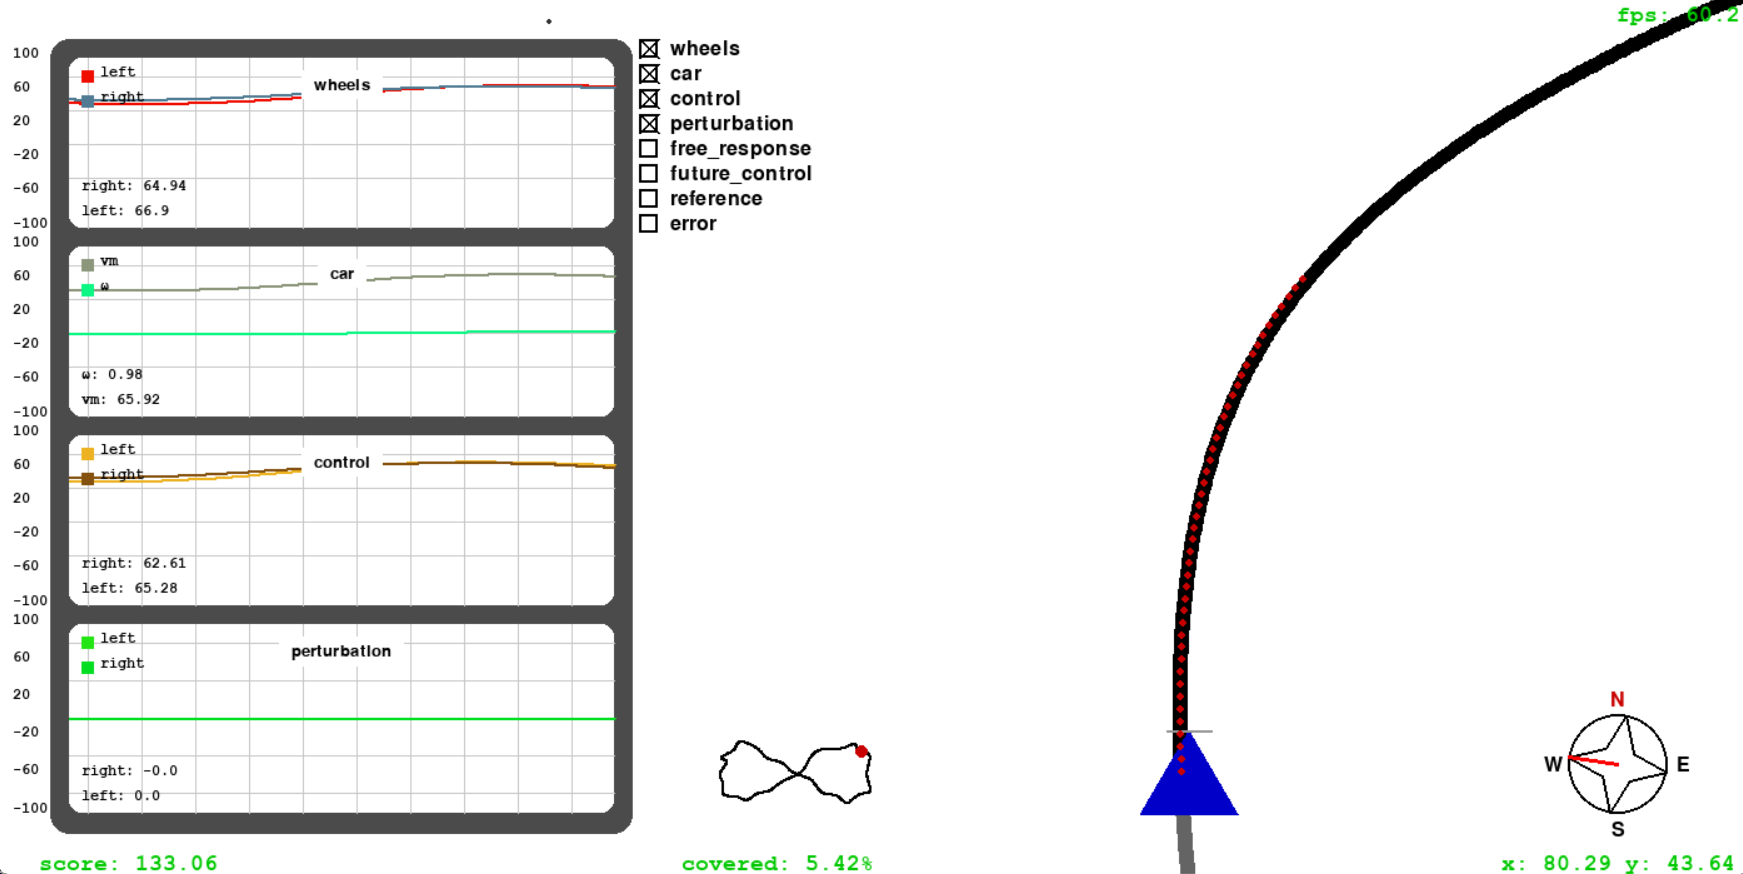
\includegraphics[width=1.0\textwidth]{figures/robot_silmulation.png}
    \caption{Interface do simulador}
    \label{fig:simulator}
\end{figure}

\vspace{1em}
Utilizando valores normalizados entre 0 a 100\% para $\mathbf{u}$,
a implementação do GPC considerou os seguintes parâmetros:

\begin{itemize}
    \item Período de amostragem $T = 0.0125$s (80fps);
    \item Horizonte de predição $N_{ss} = 5 \tau$ do motor mais lento;
    \item Horizonte de controle $M = 5$;
    \item Peso da ação de controle $\boldsymbol{\delta_e}$ e $\boldsymbol{\delta_d} = 0.001$;
    \item Peso do erro $\boldsymbol{\lambda_s} = 1$ e $\boldsymbol{\lambda_{\theta}} = 0.5$;
\end{itemize}

Os parâmetros do robô foram considerando:

\begin{itemize}
    \item Raio das rodas $r = 0.04$m;
    \item Distância entre as rodas $L = 0.15$m;
    \item Tempo de acomodação $\tau_e = 0.62$s e $\tau_d = 0.58$s;
    \item Ganho estático para $v$: $K_{ev} = 0.042$ e $K_{dv} = 0.042$;
    \item Ganho estático para $\omega$: $K_{e\omega} = 0.55$ e $K_{d\omega} = 0.55$;
\end{itemize}
